\documentclass{article}
% Change "article" to "report" to get rid of page number on title page
\usepackage{amsmath,amsfonts,amsthm,amssymb}
\usepackage{setspace}
\usepackage{Tabbing}
\usepackage{fancyhdr}
\usepackage{lastpage}
\usepackage{extramarks}
\usepackage{chngpage}
\usepackage{soul,color}
\usepackage{graphicx,float,wrapfig}
\usepackage{multirow}
\usepackage{enumerate}
% In case you need to adjust margins:
\topmargin=-0.45in      %
\evensidemargin=0in     %
\oddsidemargin=0in      %
\textwidth=6.5in        %
\textheight=9.0in       %
\headsep=0.25in         %

% Homework Specific Information
\newcommand{\hmwkTitle}{Decompose Restaurant(DR) 2}
\newcommand{\hmwkClass}{}
\newcommand{\hmwkAuthorName}{Donglai\ Wei}


% Setup the header and footer
\pagestyle{fancy}                                                       %
\lhead{\hmwkAuthorName}                                                 %
\rhead{\firstxmark}                                                     %
\lfoot{\lastxmark}                                                      %
\cfoot{}                                                                %
\rfoot{Page\ \thepage\ of\ \pageref{LastPage}}                          %
\renewcommand\headrulewidth{0.4pt}                                      %
\renewcommand\footrulewidth{0.4pt}                                      %

% This is used to trace down (pin point) problems
% in latexing a document:
%\tracingall

%%%%%%%%%%%%%%%%%%%%%%%%%%%%%%%%%%%%%%%%%%%%%%%%%%%%%%%%\begin{enumerate}

% Some tools
\newcommand{\enterProblemHeader}[1]{\nobreak\extramarks{#1}{#1 continued on next page\ldots}\nobreak%
                                    \nobreak\extramarks{#1 (continued)}{#1 continued on next page\ldots}\nobreak}%
\newcommand{\exitProblemHeader}[1]{\nobreak\extramarks{#1 (continued)}{#1 continued on next page\ldots}\nobreak%
                                   \nobreak\extramarks{#1}{}\nobreak}%

\newlength{\labelLength}
\newcommand{\labelAnswer}[2]
  {\settowidth{\labelLength}{#1}%
   \addtolength{\labelLength}{0.25in}%
   \changetext{}{-\labelLength}{}{}{}%
   \noindent\fbox{\begin{minipage}[c]{\columnwidth}#2\end{minipage}}%
   \marginpar{\fbox{#1}}%

   % We put the blank space above in order to make sure this
   % \marginpar gets correctly placed.
   \changetext{}{+\labelLength}{}{}{}}%

\setcounter{secnumdepth}{0}
\newcommand{\homeworkProblemName}{}%
\newcounter{homeworkProblemCounter}%
\newenvironment{homeworkProblem}[1][Problem \arabic{homeworkProblemCounter}]%
  {\stepcounter{homeworkProblemCounter}%
   \renewcommand{\homeworkProblemName}{#1}%
   \section{\homeworkProblemName}%
   \enterProblemHeader{\homeworkProblemName}}%
  {\exitProblemHeader{\homeworkProblemName}}%

\newcommand{\problemAnswer}[1]
  {\noindent\fbox{\begin{minipage}[c]{\columnwidth}#1\end{minipage}}}%

\newcommand{\problemLAnswer}[1]
  {\labelAnswer{\homeworkProblemName}{#1}}

\newcommand{\homeworkSectionName}{}%
\newlength{\homeworkSectionLabelLength}{}%
\newenvironment{homeworkSection}[1]%
  {% We put this space here to make sure we're not connected to the above.
   % Otherwise the changetext can do funny things to the other margin

   \renewcommand{\homeworkSectionName}{#1}%
   \settowidth{\homeworkSectionLabelLength}{\homeworkSectionName}%
   \addtolength{\homeworkSectionLabelLength}{0.25in}%
   \changetext{}{-\homeworkSectionLabelLength}{}{}{}%
   \subsection{\homeworkSectionName}%
   \enterProblemHeader{\homeworkProblemName\ [\homeworkSectionName]}}%
  {\enterProblemHeader{\homeworkProblemName}%

   % We put the blank space above in order to make sure this margin
   % change doesn't happen too soon (else \sectionAnswer's can
   % get ugly about their \marginpar placement.
   \changetext{}{+\homeworkSectionLabelLength}{}{}{}}%

\newcommand{\sectionAnswer}[1]
  {% We put this space here to make sure we're disconnected from the previous
   % passage

   \noindent\fbox{\begin{minipage}[c]{\columnwidth}#1\end{minipage}}%
   \enterProblemHeader{\homeworkProblemName}\exitProblemHeader{\homeworkProblemName}%
   \marginpar{\fbox{\homeworkSectionName}}%

   % We put the blank space above in order to make sure this
   % \marginpar gets correctly placed.
   }%

%%%%%%%%%%%%%%%%%%%%%%%%%%%%%%%%%%%%%%%%%%%%%%%%%%%%%%%%%%%%%



%%%%%%%%%%%%%%%%%%%%%%%%%%%%%%%%%%%%%%%%%%%%%%%%%%%%%%%%%%%%%
% Make title
\title{\vspace{0.3in}\textmd{\textbf{\hmwkTitle}}}
\date{2010.6.20}
\author{\textbf{\hmwkAuthorName}}
%%%%%%%%%%%%%%%%%%%%%%%%%%%%%%%%%%%%%%%%%%%%%%%%%%%%%%%%%%%%%

\begin{document}
\begin{spacing}{1.1}
\maketitle


\section{1) Algorithm (DR)}
GOAL: Maximize log Probability P=$log p(x,z|\lambda,\alpha,\gamma)$ \\ \\
\begin{enumerate}[(i)]
\item Make Restaurant j into one table t1 where customers following uniform distribution
\item Iterate until no customers are left in this uniform table t1:
\begin{enumerate}
\item For each dish k, propose to form a new table$^{1*}$ out of t1 with dish k and calculate the change $\Delta P$
\item Sample$^{2*}$ a proposal according to the weight and make the new table
\end{enumerate}
\item TKM:Local search Table/Dish(allowing new dish)+Merge dish
\item Decision$^{3*}$
\end{enumerate}

{\bf Remarks:}:\\ \\
Sampling weight:$e^{r\Delta P}$:r($>$0) is the tuning parameter(the more decrease of $\Delta P$ the less weight)\\ \\
\begin{tabular}{|c|ccc|r|}
	\hline
  &  Previous Approach   & Current Approach   \\
	\hline
$^{1*}$Form new table &Greedily assign overlapped words(threshold/not) & sampling word assignment$\sim (\dfrac{1}{W},\dfrac{n_{..k}^{w}+\phi}{n_{..k}+W\phi})$ \\ \\
$^{2*}$Sample proposal & Hard Assignment $(r_{accept}=\infty)$ & Soft Assignment:$r_{proposal}\in [0,1]$ \\ \\
$^{3*}$Decision:  & Accept all$(r_{accept}=0)$/Accept$\&$Reject$(r_{accept}=\infty)$ & Sample $r_{accept}\in [0,1]$ \\
	\hline
\end{tabular}


\newpage
\section{2) Experiment}
\subsection{i) Sampling new table proposal}
$^{1*}$ (Sampling new tables instead of Deterministic assignment)has {\bf GREAT} improvement!!!(No need for Decompose Dish any more)\\ \\
1) Hard assignment may seduce dishes to keep their mixture of bars since it has less varibility.\\
2) Sampling new table tends to try out more possibilities, which may finally break down the mixture of bars after accumulation.\\

\begin{figure}
 \centering
    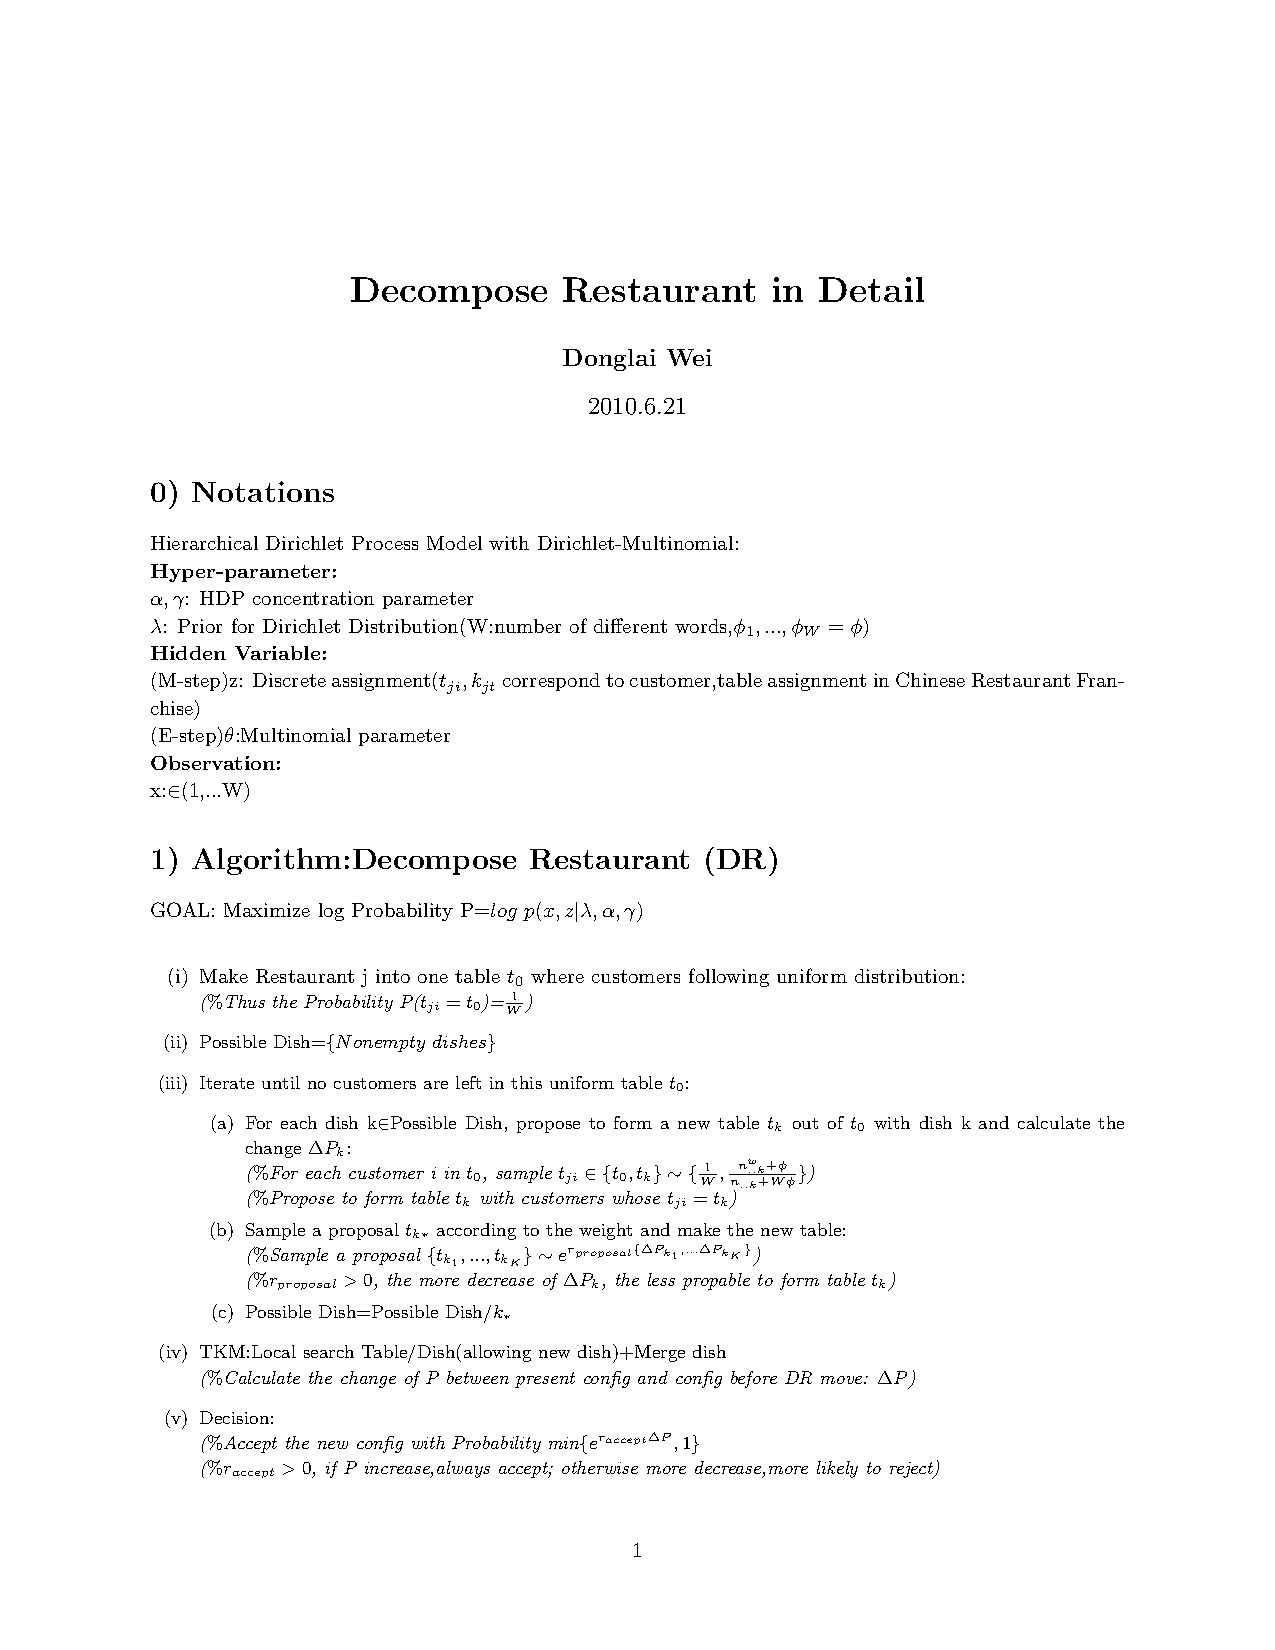
\includegraphics[width=6in,height=5in]{sample.pdf} 
    \caption{With same set of parameters,sampling new table assignment(right column) is much better than deterministic(greedy) ones(left,mid column)}
    \label{fig:by:table} 
\end{figure}



\newpage
\subsection{ii)Comparison of 2 strategies}
(Below, algorithms all use Sampling new table assignment in$^{*1}$)\\ \\ \\
a) Peaky new table Proposal($r_{proposal}\sim$1)+More Acceptance($r_{accept}<<$1)\\ \\ \\
{\bf Good:}\\ 
1) Quickly shrink the number of dishes:\\
In the beginning, every restaurant is its own dish. Peaky proposal greedily try out one searching direction instead of wasting time wandering around.
Decompose restaurant tends to interpret the restaurant with more dishes which may decrease $\Delta P$ to vary degrees. Thus we should be 
more tolerant during Initialization.\\ \\
{\bf Bad:}\\ \\
1) Maybe vulnerable to local optima, since it's lack of variability\\
2) Don't know when to stop\\ \\
{\bf Further Remarks:}\\ \\
1)I also go to extremes that: Find the best new table Proposal+Accept All, which works equally well. So I guess the variability in $^{*1}$(sampling) is enough and
the greedy decision maynot be too bad to be rejected.\\
2)Though it finds 10 bars quickly, $P$ is still a little lower than some of the noisy configurations.(More DR runs with Accept/Reject needed,guaranteed to decrease)

\begin{figure}
 \centering
   \begin{tabular}{cc}    
     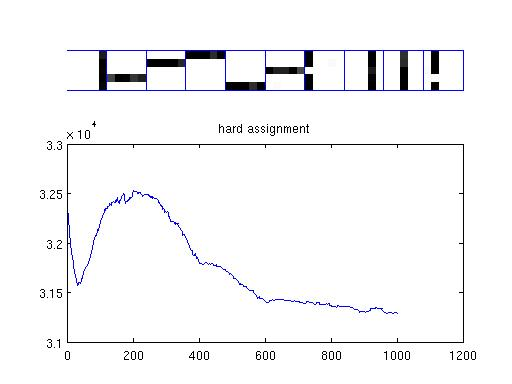
\includegraphics[width=3in,height=2.5in]{200_hard.jpg} &
     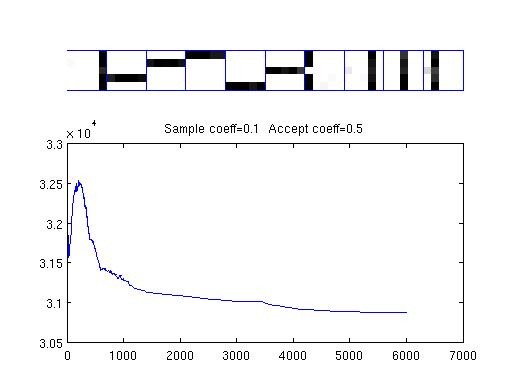
\includegraphics[width=3in,height=2.5in]{200_hard_stuck.jpg} \\
   \end{tabular}
    \caption{(left)is the initial 5 DR strategy a)moves;(right)More DR strategy a)runs with Accept/Reject}
    \label{fig:by:table} 
\end{figure}

\begin{figure}
 \centering
    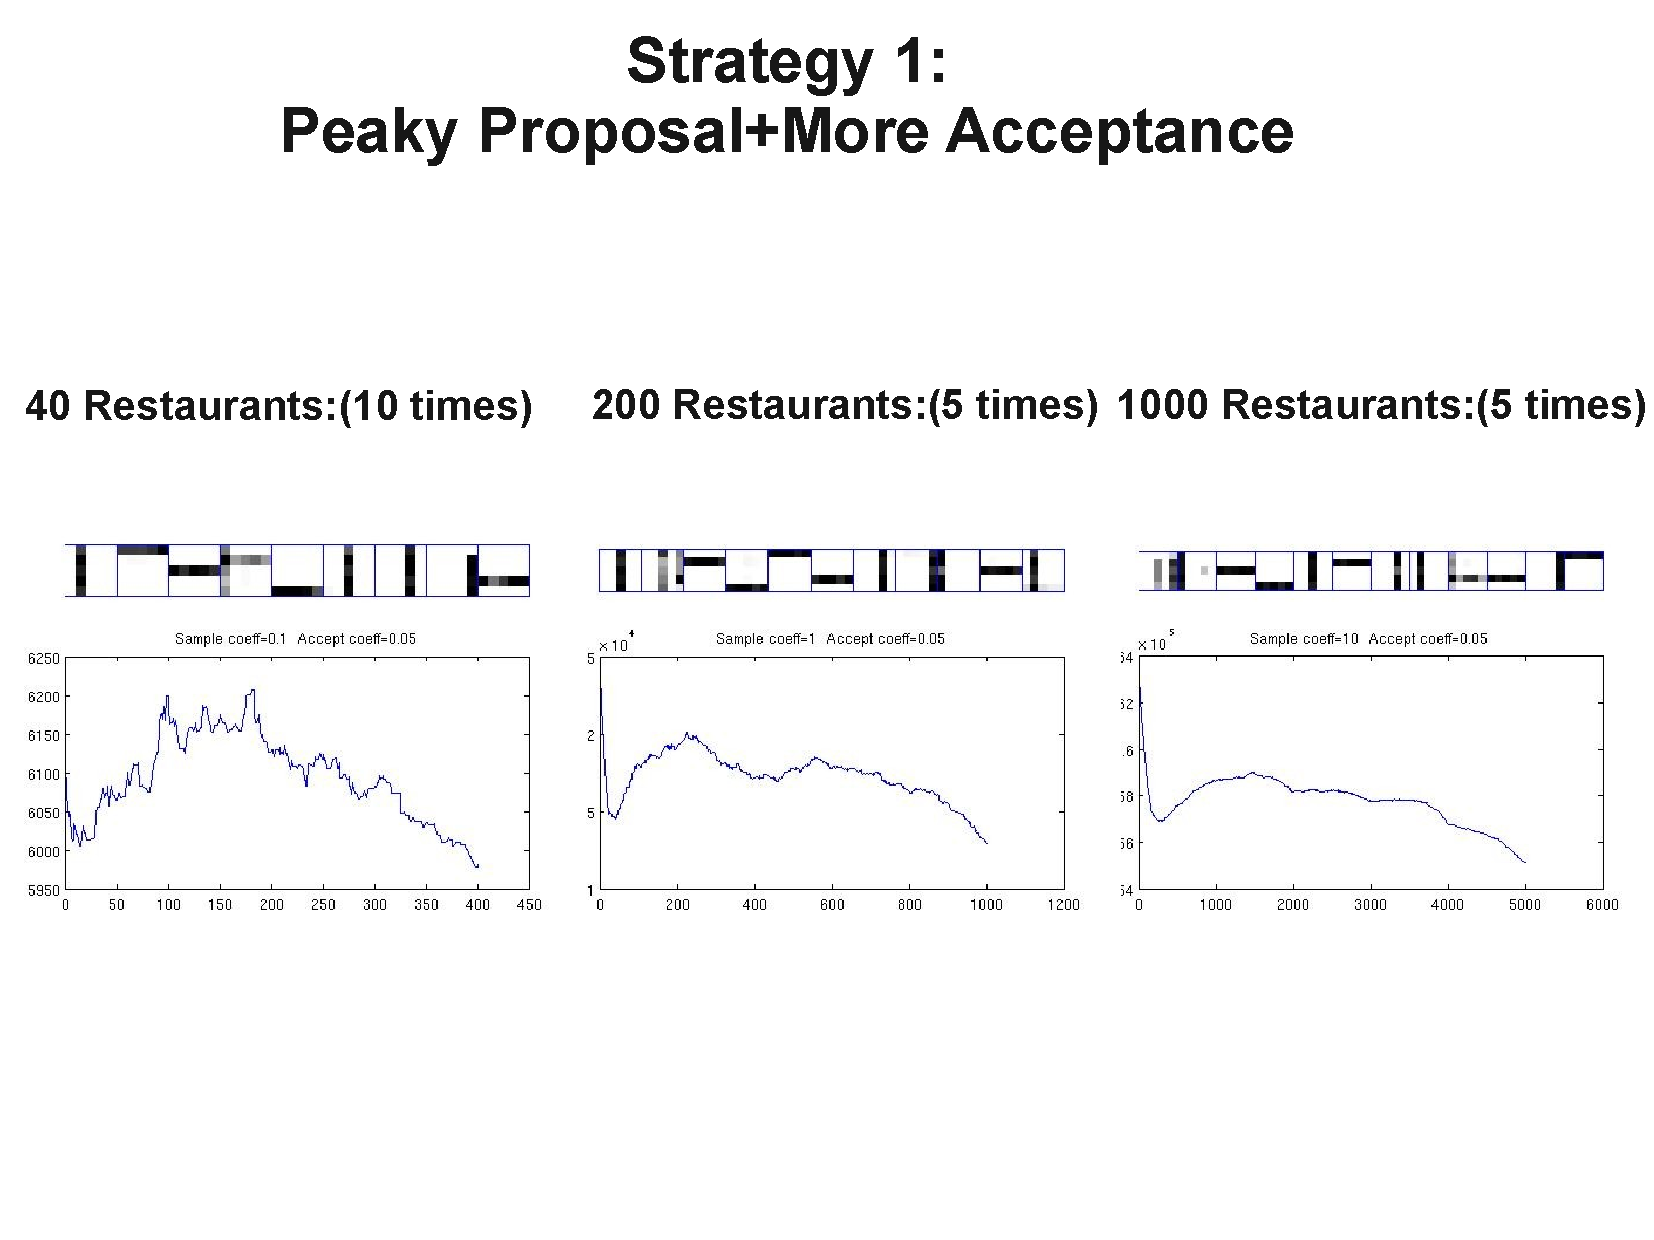
\includegraphics[width=6in,height=5in]{strategy_2.pdf} 
    \caption{A set of parameters that Peaky new table proposal+More Acceptance work}
    \label{fig:by:table} 
\end{figure}
\newpage
b) Flatter Proposal($r_{proposal}<<$1)+Less Acceptance($r_{accept}\sim$1)\\ \\ \\
{\bf Good:}\\ 
1) More variability during the search:\\
Since the chance to get "worse"(in terms of long-term searching direction) config increases, we need sharper Acceptance Decision.\\ \\
{\bf Bad:}\\ 
1) Too Slow to reduce the number of dishes, since it wastes lots of time wondering around.\\
2) Tend to have noisy dishes: Since the Acceptance Decision is sharper, many of the potential "better" config(tendency to break down the noisy dish) are rejected,
leaving dishes nasty.\\ \\
{\bf Further Remarks:}\\ 
1)Though it is hopeless to find 10 bars(I tried more iterations), it has equally good $P$. Bigger tables and Noisy dishes maynot be a bad interpretation in terms of $P$\\
\begin{figure}
 \centering
   \begin{tabular}{cc}    
     \resizebox{60mm}{!}{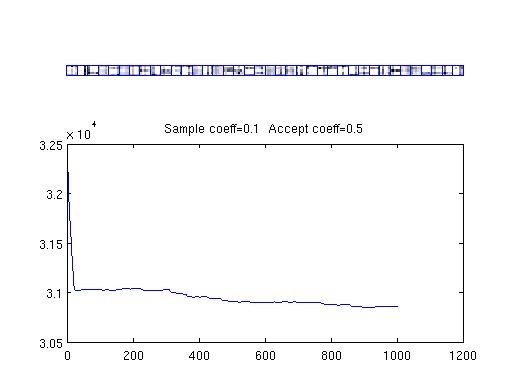
\includegraphics{200_01_05.jpg}} &
     \resizebox{60mm}{!}{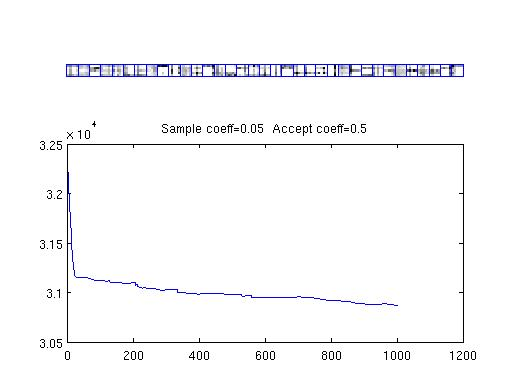
\includegraphics{200_005_05.jpg}} \\
   \end{tabular}
    \caption{Flatter Proposal+Less Acceptance: the $P$ is really good}
    \label{fig:by:table} 
\end{figure}


\end{spacing}
\end{document}

%%%%%%%%%%%%%%%%%%%%%%%%%%%%%%%%%%%%%%%%%%%%%%%%%%%%%%%%%%%%%
